%%%%%%%%%%%%%%%%%%%%%%%%%%%%%%%%%%%%%%%%%%%%%%%%%%%%%%%%%%%%%%%%%%%%%%%%
% Preamble
%%%%%%%%%%%%%%%%%%%%%%%%%%%%%%%%%%%%%%%%%%%%%%%%%%%%%%%%%%%%%%%%%%%%%%%%
\documentclass[11pt]{article}
%
% Packages and other includes
% Pagination
\usepackage[letterpaper, margin=1in]{geometry}
\usepackage{emptypage}
\usepackage{ulem}
\usepackage{xcolor}
\usepackage{mhchem}
%
% Fonts
\usepackage[T1]{fontenc} % best for Western European languages
\usepackage{lmodern} % Latin Modern instead of CM
\usepackage{textcomp} % required to get special symbols
%
% Math
\usepackage{amsmath, amssymb}
\usepackage{braket}
%
% Graphics, floats, tables
\usepackage{graphicx, color, float, array}
%
% Hyperlinks
\usepackage{hyperref}
%
%
% Definitions and settings
% Paragraph indent and spacing
\setlength{\parskip}{0.4\baselineskip}
\setlength{\parindent}{0in}
%
%
% Title, authors, date
\title{\textbf{Worksheet 9}}
\date{\vspace{-2em}March 4th, 2022}
%
%
%%%%%%%%%%%%%%%%%%%%%%%%%%%%%%%%%%%%%%%%%%%%%%%%%%%%%%%%%%%%%%%%%%%%%%%%
% Main document
%%%%%%%%%%%%%%%%%%%%%%%%%%%%%%%%%%%%%%%%%%%%%%%%%%%%%%%%%%%%%%%%%%%%%%%%
%

\begin{document}

\maketitle

Collaborations are encouraged and students must report all collaborators
on each assignment. All external sources (websites, books) must be
cited. An \textit{extra credit} (\textit{EC}) problem will be available per
assignment. Please submit a completed homework on-time to receive \textit{EC}
and no partial \textit{EC} (all parts must be correct) will be given out.
Additional problems are listed at the end of each assignment. This week's
assignment is due \textit{Monday, March 14th at 10:30am.}

1. \textbf{Concentrations of Solutions} An car antifreeze mixture is made by mixing
equal volumes of ethylene glycol (d = 1.114 g/mL, molar mass 62.07 g/mol) and water
(d = 1.000 g/mL) at 20.0$^\circ$C. The density of the solution is 1.070 g/mL. Determine
the mass percent, molarity, molality, and mole fraction.

%https://www.chemteam.info/Solutions/Molality-molarity-density-mass-precent-mole-ratio-Prob11-25.html

2. \textbf{Henry's Law} The Henry's law says that the amount of dissolved gas in
a given volume of solvent at equilibrium is proportional to the partial pressure of
the gas. 
\begin{equation}
  c(\text{solute}) = k_HP(\text{solute})
\end{equation}
The minimum mass concentration of oxygen O$_2$ required for fish life is 4.0 mg/L.
Henry's constant for O$_2$ is $1.2\times 10^{-3}$ mol/(L atm). Report results to 2
significant figures.

(a) Assume the density of lake water to be 1.00 g/mL and express this concentration
in parts per million (milligrams of O$_2$ per kilogram of water mg/kg).

(b) What is the minimum partial pressure of O$_2$ that would supply the minimum mass
concentration of oxygen in water to support fish life at 20.$^\circ$C.

(c) What is the minimum atmospheric pressure that would give this partial pressure,
assuming that oxygen exerts about $21\%$ of the atmospheric pressure?

% Atkins 9.27

3. \textbf{Raoult's Law} 

4. \textbf{Freezing Point Depression} When 1.32g of a nonpolar solute was dissolved in
50.0g of phenol, the latter's freezing point was lowered by 1.454$^\circ$C. Calculate
the molar mass of the solute. Phenol $K_f = 7.40^\circ/m$

\pagebreak

5. \textbf{Colligative Properties of Solution} Two beakers, one containing 0.10 m NaCl(aq)
and the other containing 0.010 m AlCl$_3$(aq), are placed inside a bell jar and sealed.
The beakers are left unitl the water vapor has come to equilibrium with any liquid in the
container. The levels of the liquid in each beaker at the beginning of the experiment
are the same, as pictured in Fig. \ref{fig:beakers}. Draw the levels of the liquid in
each beaker after quilibrium has been reached. Explain your reasoning.

\begin{figure}[hbpt]
  \centering
  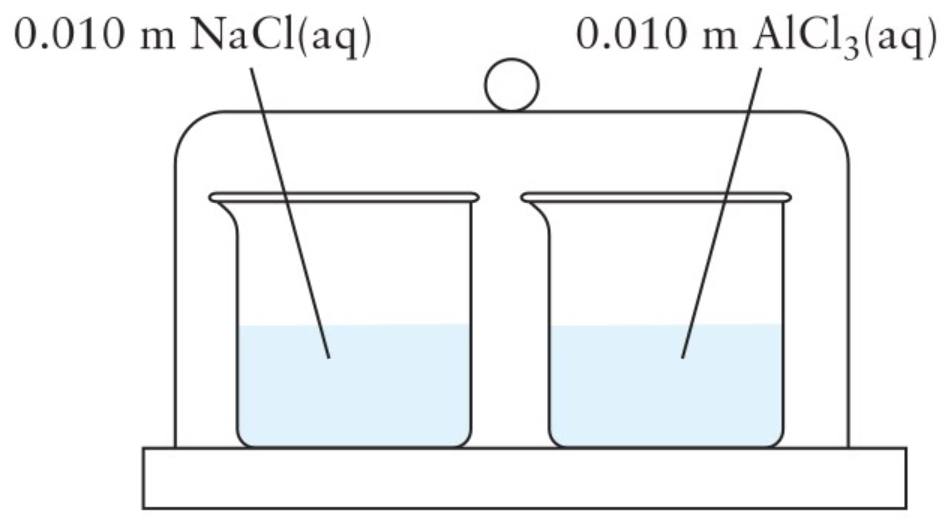
\includegraphics[scale=0.3]{nacl_alcl3.png}
  \caption{0.010 m NaCl and 0.010 m AlCl$_3$ are separated in equal sized
    containers.}
  \label{fig:beakers}
\end{figure}

6. \textbf{Solid Structures} Determine the number of atoms per unit cell,
see Fig. \ref{fig:cub}.

\begin{figure}[hbpt]
  \centering
  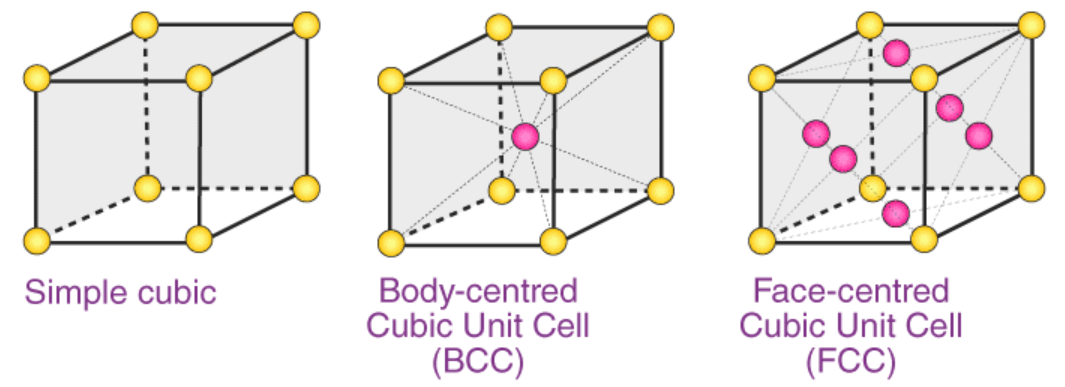
\includegraphics[scale=0.3]{cubic.png}
  \caption{Various solid structures}
  \label{fig:cub}
\end{figure}

\vfill
\textbf{Optional Additional Problems:} Ch. 12 - odd problems $25 - 47$, $79 - 85$;
Ch. 13 - odd problems $25 - 35$, $47 - 55$, $65 - 93$

\end{document}
